\section{Optimizations}
\subsection{Efficient Separation}
The \gls{volta} has 48KiB of available shared memory per block \cite{rigerunNVIDIAJetsonXavier2023}.
With an image width of 2448 pixels \cite{lucidvisionlabsTriton0MPPolarization} it is only possible to store 10 lines in local shared memory as each pixel uses 16 bits.
\begin{equation*}
    \frac{48Kib}{2448px/line * 16b/px} = \frac{393216b}{39168b/line} \approx 10.04line
\end{equation*}

In order to allocate local memory for prefetching, it became necessary to reduce the amount of image data stored in local memory.
This challenge was overcome by recognizing that the transformation process for even and odd lines is independent and identical.
As illustrated in Figure \ref{fig:saperation}, the even and odd lines can be separated, allowing two thread blocks to process each part independently.

It is important to highlight that the updated \jo now supports a maximum of $163KiB$ of local memory per thread block, rendering this separation unnecessary if utilized \cite{CUDA2023}.
\begin{figure}[H]
    \centering
    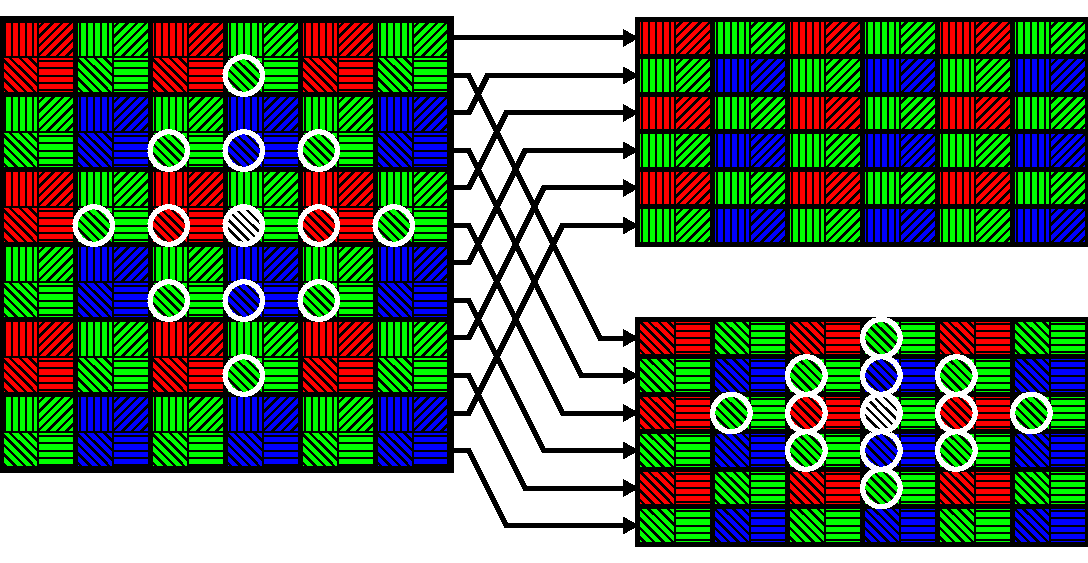
\includegraphics[width=.8\textwidth]{figures/polarized_image/separation.pdf}
    \caption{How separation is done in order to reduce the amount of shared memory required per thread block.}
    \label{fig:saperation}
\end{figure}

\subsection{Array Rotation and Concurrent Prefetching}
The current \gls{mhc} method requires six lines of the image to be available in local memory for the convolution process.
The local memory is structured as an array of pointers to local line data, making it possible to rotate the array after each convolution, as shown in Figure \ref{fig:reuse}.

\begin{figure}[H]
    \centering
    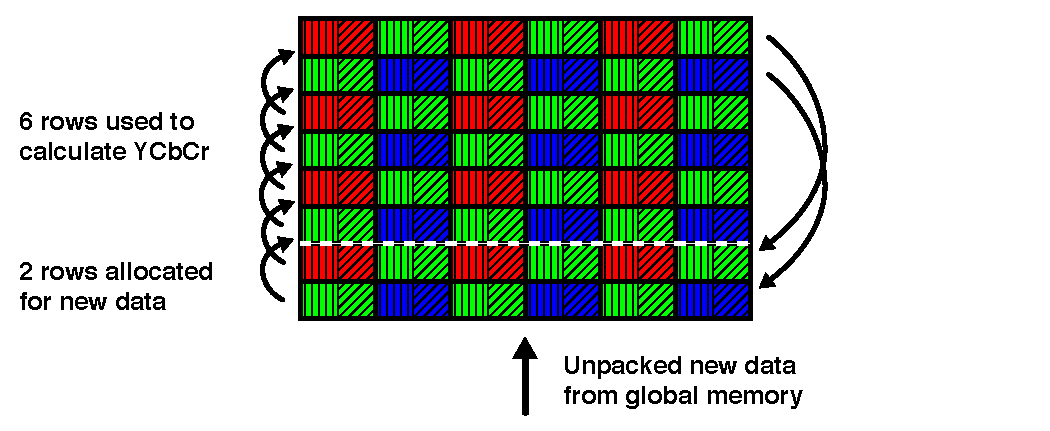
\includegraphics[width=\textwidth]{figures/polarized_image/rolling.pdf}
    \caption{Visualization of image rotation.}
    \label{fig:reuse}
\end{figure}

The local memory has eight rows, such that while computation is performed on the first six rows, the next two rows can be prefetched from global memory and unpacked.
This is done by a separate group of warps, enabling concurrent computation and prefetching, as shown in Figure \ref{fig:saperation}.


\begin{figure}[H]
    \centering
    \subcaptionbox{Initial implementation.}{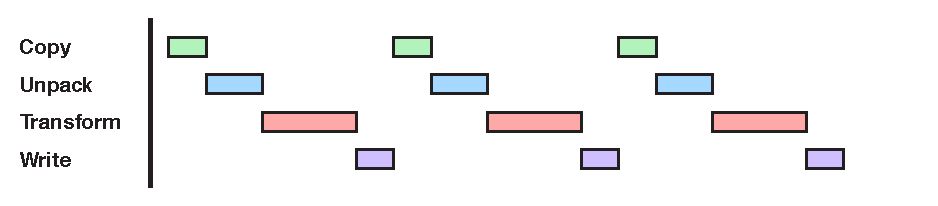
\includegraphics[width=\textwidth]{figures/debayer/debayer_non_concurrent.pdf}}
    \subcaptionbox{Current implementation.}{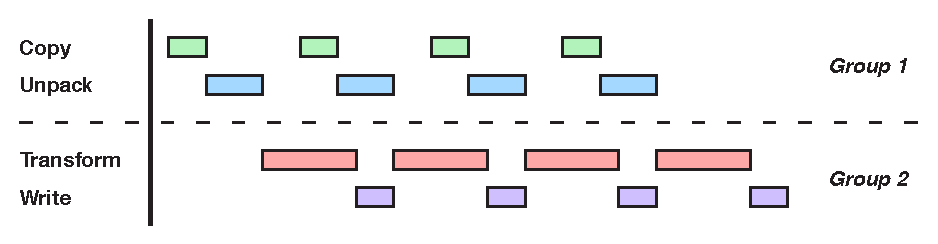
\includegraphics[width=\textwidth]{figures/debayer/debayer_concurrent.pdf}}
    \caption{Concurrent computation and prefetching.}
    \label{fig:saperation}
\end{figure}



